\chapter{Augmented Lagrangian Method}
\label{cha:2}
In this chapter the direct multiple shooting approach is examined more closely and a more specific algorithm is designed to replace \texttt{fmincon}, which is a very general method. For this problem the Augmented Lagrangian Method has been chosen. It will be implemented in python using \texttt{numpy},\texttt{scipy}, and \texttt{keras}

\section{Augmented Lagrangian Method}
TODO: cite textbook, 1906


Instead of using fmincon, now an Augmented Lagrangian Method (ALM) is used to solve the Optimal Control Problem (OCP). The OCP is described in equation \ref{ocp-eq} and is printed here again:
\begin{equation*}
	\begin{aligned}
	& \underset{W}{\text{minimize}}
	& & \frac{1}{2}\sum\limits_{j=0}^{N}||W_Hz_H^j - y^j||^2 \\
	& \text{subject to} \\
	& & 0 &= x_0 - \sigma(W_0x_0^j + b_0) &j = 1,\ldots,N \\
	& & 0 &= z_{k+1}^j - \sigma(W_kx_k^j + b_k), &k = 0,\ldots,H-1,j = 1,\ldots,N
	\end{aligned}
\end{equation*}

This is a nonlinear least squares problem:

\begin{equation*}
	\begin{aligned}
	& \text{min}
	&  & \frac{1}{2} ||F(x)||^2_2 \\
	& \text{s. t.}
	& &  h(x) = 0
	\end{aligned}
\end{equation*}

The ALM is designed to solve this sort of problem. It constructs an unconstrained problem by adding the constraints in both a penalty and a lagrangian term. The lagrangian cost function looks like this:

\begin{equation}
\mathcal{L}_c(x,\lambda) = \frac{1}{2} ||F(x)||^2_2 + <\lambda,h(x)> + \frac{c}{2} || h(x) ||^2_2
\end{equation}

where c is a penalty term, and $\lambda$ are the lagrangian parameters. The algorithm consists of an inner and outer loop. In the inner loop of the algorithm $\mathcal{L}_c{x,\lambda}$ is minimized for $x^k$ up to a certain tolerance.

\begin{equation}
	\begin{aligned}
	 & \underset{x}{\text{min}} & \mathcal{L}_c(x,\lambda) 
	     &= \frac{1}{2} ||F(x)||^2_2 + <\lambda,h(x)> + \frac{c}{2} || h(x) ||^2_2 \\
	 & & &= \frac{1}{2} ||F(x)||^2_2 + \frac{c}{2} ||h(x) + \lambda/c ||^2_2 - \frac{1}{2c} ||\lambda||^2_2 \\
	 & & &= \frac{c}{2} \Big|\Big|
		\begin{bmatrix}
			F(x)/\sqrt{c} \\
			h(x) + \lambda/c
		\end{bmatrix} \Big|\Big|^2_2 \\
	 & & &= \frac{c}{2} ||G_c(x,\lambda)||^2_2
	\end{aligned}
	\label{loss}
\end{equation}

Where $G_c$ is defined as the function within the square norm. This is a nonlinear least squares problem which is solved by the \texttt{least\_squares} procedure implemented in the python package \texttt{scipy.optimize}. The function insid until the norm of the gradient of $G_c$ meets a certain tolerance $\epsilon$:

\begin{equation}
|| \nabla_kG_{c_k}(x^k,\lambda^k)||_2 \leq \epsilon
\end{equation}
 
where k is the current iterate and $\lambda^k$ are the current lagrangian parameters. The Jacobian matrix $J = \nabla_kG_{c_k}^T$ is calculated analytically and analysed further in the next section. The Langrangian parameters $\lambda^k$ are then updated in each iteration using this rule:

\begin{equation}
\lambda^{k+1} = \lambda^k + c_kh(x^k)
\end{equation}

A new penalty parameter $c^{k+1}$ are updated using the rule described in \cite{}, which depends on the norm of the gradient. If the constraints are sufficiently respected, the penalty parameter is not updated, otherwise the penalty parameter is increased by a factor 100. The algorithm continues in this manner until the norm of the Jacobian matrix reaches a tolerance $\zeta$.


\begin{equation}
	\begin{aligned}
		\mathcal{L}_c(x,\lambda)
		&= \frac{1}{2} ||F(x)||^2_2 + <\lambda,h(x)> + \frac{c}{2} || h(x) ||^2_2 \\
		&= \frac{1}{2} ||F(x)||^2_2 + \frac{c}{2} ||h(x) + \lambda/c ||^2_2 - \frac{1}{2c} ||\lambda||^2_2 \\
		&= \frac{c}{2} \Big|\Big|
		\begin{bmatrix}
			F(x)/\sqrt{c} \\
			h(x) + \lambda/c
		\end{bmatrix} \Big|\Big|^2
	\end{aligned}
	\label{loss}
\end{equation}

\begin{figure}
     \centering
     \begin{subfigure}[b]{0.8\textwidth}
         \centering
         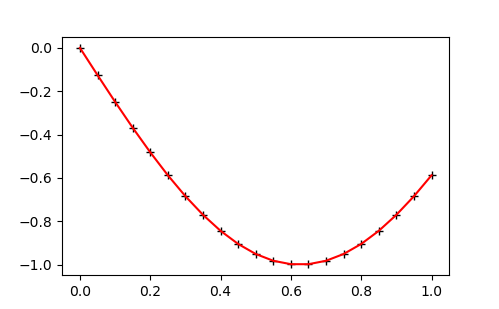
\includegraphics[width=\textwidth]{alm-tanh}
         \caption{Training performance of simultaneous approach, with tansig activation function}
         \label{alm-tanh}
     \end{subfigure}
     \begin{subfigure}[b]{0.8\textwidth}
         \centering
         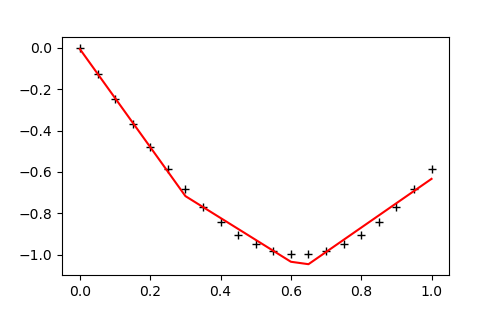
\includegraphics[width=\textwidth]{alm-relu}
         \caption{Training performance of simultaneous approach, with ReLU activation function}
         \label{alm-relu}
     \end{subfigure}
     \begin{subfigure}[b]{0.8\textwidth}
         \centering
         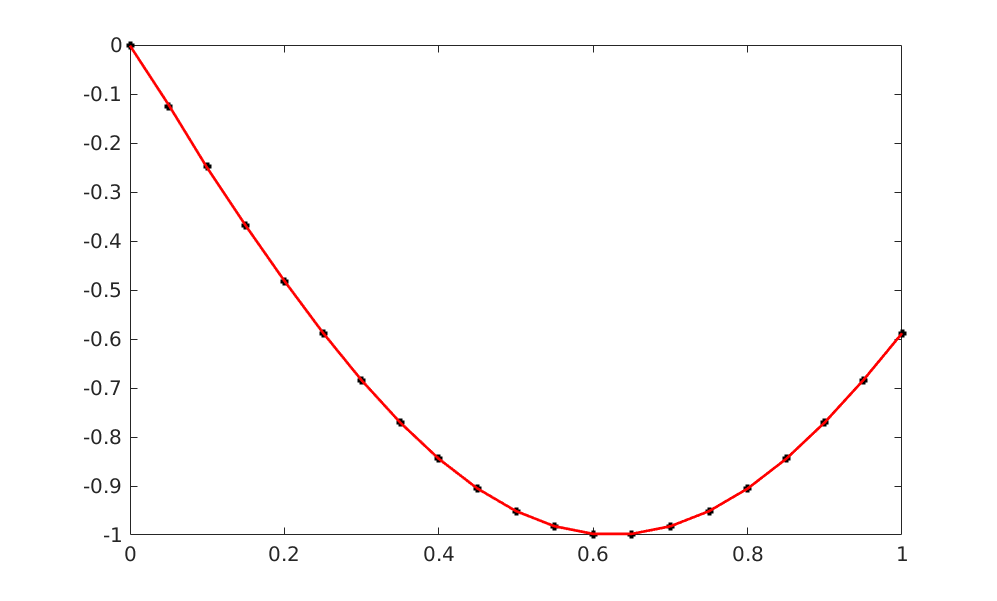
\includegraphics[width=\textwidth]{back-relu}
         \caption{Training performance of backpropagation, with ReLU activation function}
     \end{subfigure}
        \caption{Performance of algorithms for simple regression problem}
        \label{back-relu}
\end{figure}

\section{Jacobian}
To solve the least squares problem, the Jacobian matrix must be calculated. It has a relatively sparse structure because there are no distant connections in the neural net, each layer is only connected to the next one and the previous one.

Neural networks obviously have many possible architectures, so a simple fully connected rectangular feedforward network is considered. It has an input dimension I, an output dimension O, and it has D hidden layers of width W. The weight matrixes have $I\times W + O\times W + (D-1)\times W\times W$ parameters, the bias vectors have $D\times W+O$ parameters and the state vectors have $D\times W\times N$ parameters. On the other hand $\mathcal{L}_c(x,\lambda)$ will have an output dimension of $D\times W \times N + O\times N$. The dimension of the Jacobian will be $(D \times W\times N + O\times N)\times (D\times W\times N + O + (D+I+O)\times W + (D-1)\times W^2)$. Therefore the Jacobian will be taller than it is wide when $N \geq 1 + (D+I+O)\times W/O + (D-1)\times W^2/O$. Written out completely the Jacobian will look like Table \ref{jac-tab}

\newpage
\begin{adjustwidth}{2000pt}{2000pt}
\begin{table}
\tiny
\centering
\begin{tabular}{r r | c c c c c}\hline

& $\nabla\mathcal{L}$ & $W_{0_1}$ & $W_{0_2}$ & ... & $W_{0_W}$ & $b_0$ \\
& & I & I &...& I & W \\ \hline
$F$ & O*N & 0 & 0 &...& 0 & 0\\ \hline
$h_1$ & N & 		$-x\sigma'(W_{0_1}x+b_{0_1})$ & 0 &...& 0 & $-\sigma'(W_{0_1}x+b_{0_1})$ \\
      & N & 0 & 	$-x\sigma'(W_{0_2}x+b_{0_2})$ &...& 0 &  	$-\sigma'(W_{0_2}x+b_{0_2})$ \\
      &...&...&...&...&...&... \\
      & N & 0 & 0 &...& $-x\sigma'(W_{0_W}x+b_{0_W})$ &  		$-\sigma'(W_{0_W}x+b_{0_W})$ \\ \hline
$h_2$ & W*N & 0 & 0 &...& 0 & 0 \\
...   & ... &...&...&...&...&...\\ 
$h_{D}$ & W*N & 0 & 0 &...& 0 & 0 \\ \hline \\ \hline

& $\nabla\mathcal{L}$ & $W_{i_1}$ & $W_{i_2}$ &...& $W_{i_W}$ & $b_1$ \\
& & W & W &...& W & W \\ \hline
$F$ & O*N & 0 & 0 &...& 0 & 0 \\ \hline
$h_1$ & W*N & 0 & 0 &...& 0 & 0 \\
...   & ... &...&...&...&...&...\\ \hline
$h_{i+1}$ & N & 		$-z_1\sigma'(W_{i_1}z + b_{i_1})$ & 0 &...& 0 & $-\sigma'(W_{i_1}x+b_{i_1})$ \\
      & N & 0 & 	$-z_1\sigma'(W_{i_2}z + b_{i_2})$ &...& 0 & 	$-\sigma'(W_{i_2}x+b_{i_2})$ \\
      &...&...&...&...&...&... \\
      & N & 0 & 0 &...& $-z_1\sigma'(W_{i_W}z + b_{i_W})$ & 		$-\sigma'(W_{i_W}x+b_{i_W})$ \\ \hline
...   & ... &...&...&...&...&...\\ 
$h_{D}$ & W*N & 0 & 0 &...& 0 & 0 \\ \hline \\ \hline

& $\nabla\mathcal{L}$ & $W_{D_1}$ &  $W_{D_2}$  &...&  $W_{D_O}$ & $b_D$ \\
& & W & W &...& W & O \\ \hline
$F$ & N & $-\frac{z_D}{\sqrt{c}}\sigma_O'(W_{D_1}x+b_{D_1})$ & 0 &...& 0 & $-\frac{1}{\sqrt{c}}\sigma_O'(W_{D_1}x+b_{D_1})$ \\
    & N & 0 & $-\frac{z_D}{\sqrt{c}}\sigma_O'(W_{D_2}x+b_{D_2})$ &...& 0 & $-\frac{1}{\sqrt{c}}\sigma_O'(W_{D_2}x+b_{D_2})$ \\
      &...&...&...&...&...&... \\
    & N & 0 & 0 &...& $-\frac{z_D}{\sqrt{c}}\sigma_O'(W_{D_O}x+b_{D_O})$ & $-\frac{1}{\sqrt{c}}\sigma_O'(W_{D_O}x+b_{D_O})$ \\ \hline
$h_1$ & W*N & 0 & 0 &...& 0 & 0 \\
...   & ... &...&...&...&...&...\\ 
$h_{D}$ & W*N & 0 & 0 &...& 0 & 0 \\ \hline
      
\end{tabular}

Square Diagonal Matrices

\begin{tabular}{ r r | c c c c }
& $\nabla\mathcal{L}$ & $z_{i_1}$ & $z_{i_2}$ &...& $z_{i_W}$\\
& & N & N &...& N \\ \hline
$F$ & O*N & 0 & 0 &...& 0 \\ \hline
$h_1$ & W*N & 0 & 0 &...& 0 \\
...   & ... &...&...&...&...\\\hline
$h_i$ & N & 1 & 0 &...& 0 \\
      & N & 0 & 1 &...& 0  \\
      &...&...&...&...&...\\ 
      & N & 0 & 0 &...& 1  \\ \hline
$h_{i+1}$ & N & $-W_{i_{1,1}}\sigma'(W_{i_1}z_i+b_{i_1})$ & $-W_{i_{1,2}}\sigma'(W_{i_1}z_i+b_{i_1})$ &...& $-W_{i_{1,W}}\sigma'(W_{i_1}z_i+b_{i_1})$\\
          & N & $-W_{i_{2,1}}\sigma'(W_{i_2}z_i+b_{i_2})$ & $-W_{i_{2,2}}\sigma'(W_{i_2}z_i+b_{i_2})$ &...& $-W_{i_{2,W}}\sigma'(W_{i_2}z_i+b_{i_2})$\\
      &...&...&...&...&...\\ 
          & N & $-W_{i_{W,1}}\sigma'(W_{i_W}z_i+b_{i_W})$ & $-W_{i_{W,2}}\sigma'(W_{i_W}z_i+b_{i_W})$ &...& $-W_{i_{W,W}}\sigma'(W_{i_W}z_i+b_{i_W})$\\ \hline
...   & ... &...&...&...&...\\ 
$h_{D}$ & W*N & 0 & 0 &...& 0 \\ \hline \\
& $\nabla\mathcal{L}$ & $z_{D_1}$ & $z_{D_2}$ &...& $z_{D_W}$\\
& & N & N & ... &  N \\ \hline
F & N &         $-W_{D_{1,1}}\sigma_O'(W_{D_1}z_D+b_{D_1})$ & $-W_{D_{1,2}}\sigma_O'(W_{D_1}z_D+b_{D_1})$ &...& $-W_{D_{1,W}}\sigma_O'(W_{D_1}z_D+b_{D_1})$\\
          & N & $-W_{D_{2,1}}\sigma_O'(W_{D_2}z_D+b_{D_2})$ & $-W_{D_{2,2}}\sigma_O'(W_{D_2}z_D+b_{D_2})$ &...& $-W_{D_{2,W}}\sigma_O'(W_{D_2}z_D+b_{D_2})$\\
      &...&...&...&...&...\\ 
          & N & $-W_{D_{O,1}}\sigma_O'(W_{D_O}z_D+b_{D_O})$ & $-W_{D_{O,2}}\sigma_O'(W_{D_O}z_D+b_{D_O})$ &...& $-W_{D_{O,W}}\sigma_O'(W_{D_O}z_D+b_{D_O})$\\ \hline
$h_1$ & W*N & 0 & 0 &...& 0 \\
...   & ... &...&...&...&...\\\hline
$h_D$ & N & 1 & 0 &...& 0 \\
      & N & 0 & 1 &...& 0  \\
      &...&...&...&...&...\\ 
      & N & 0 & 0 &...& 1  \\ \hline
\end{tabular}
\caption{Jacobian of feedforward neural network}
\label{jac-tab}

\end{table}

\end{adjustwidth}
\begin{figure}[p]
  \centering
  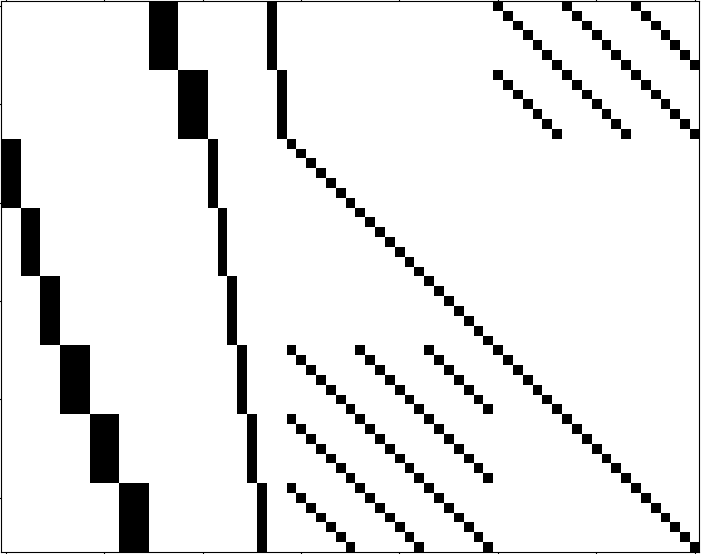
\includegraphics[width=\textwidth]{jac.png}
  \caption{Nonzero elements of Jacobian, for network with I=2,O=2,W=3,D=2,N=7}
  \label{jac}
\end{figure}

\section{Algorithmic Verification of Jacobian}
The Jacobian in the previous section was derived by hand. In this section will be explained how the Jacobian was verified algorithmically.

By Algorithmic Differentation the numerical value for the Jacobian can be deduced. For this the AlgoPy python module was used. By adding code from this packet to the calculation of the neural network, the Jacobian is calculated along with the network. This result was then compared to the analytical result for a number of different network configurations, confirming them to be equal within a small tolerance. The code is available at https://github.com/jan-scheers/thesis 

\section{Alternative Representation}

In this section we explain an alternative representation which is mathematically the same. Figure \ref{jac2} shows the Jacobian, but with the rows corresponding to the loss function put at the bottom. It shows a diagonal structure, because each layer in this feedforward net is only connected to the adjacent layers.

\begin{figure}[p]
  \centering
  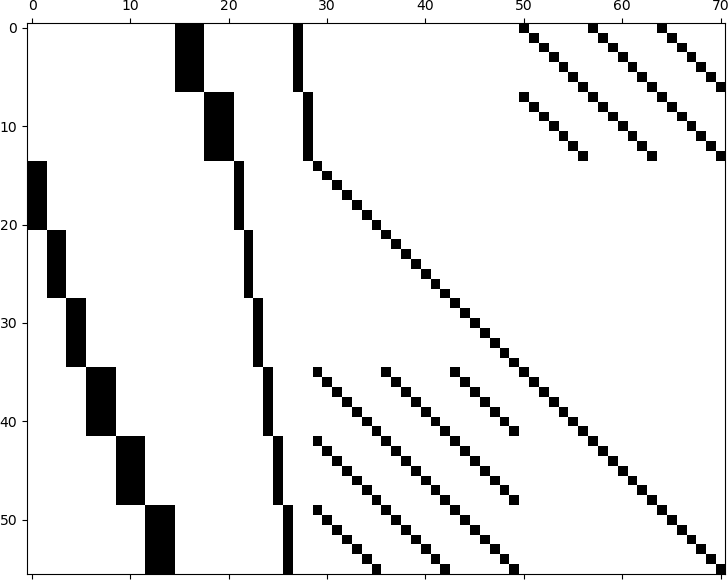
\includegraphics[width=\textwidth]{jac2.png}
  \caption{Nonzero elements of Jacobian, for network with I=2,O=2,W=3,D=2,N=7, rearranged}
  \label{jac2}
\end{figure}

\section{Testing}

In this section the tests from the previous chapter are run again, this time using the ALM algorithm. The least squares problem in the inner loop is solved using the \texttt{least\_squares} method in \texttt{numpy 1.20.1}, which is provided with the Jacobian calculated in the previous section. This time the stopping criterion is that the cost function described in equation \ref{loss} is less than a tolerance of $1e^{-6}$. Figure \ref{alm-tanh} and Figure \ref{alm-relu} show the result of these two tests.